% \iffalse meta-comment
%
% Transformed from veryshortguide.xml by ClassPack db2dtx.xsl
% version 1.19 (2020-05-19) on Thursday 21 May 2020 at 11:55:35
%
% veryshortguide.dtx is copyright © 2009-2020 by Peter Flynn <peter@silmaril.ie>
%
% This work may be distributed and/or modified under the
% conditions of the LaTeX Project Public License, either
% version 1.3 of this license or (at your option) any later
% version. The latest version of this license is in:
%
%     http://www.latex-project.org/lppl.txt
%
% and version 1.3 or later is part of all distributions of
% LaTeX version 2005/12/01 or later.
%
% This work has the LPPL maintenance status ‘maintained’.
% 
% The current maintainer of this work is Peter Flynn <peter@silmaril.ie>
%
% This work consists of the files veryshortguide.dtx and veryshortguide.ins,
% the derived file , 
% and any other ancillary files listed in the MANIFEST.
%
% \fi
% \iffalse
%<*driver>
\ProvidesFile{veryshortguide.dtx}
%</driver>
%<class>\NeedsTeXFormat{LaTeX2e}[2015/01/01]
%<class>\ProvidesClass{veryshortguide}[2020/04/16 v0.7
%<class>  The Very Short Guide to LaTeX]
%<*driver>
\RequirePackage{fix-cm}% included by default.
\PassOptionsToPackage{svgnames}{xcolor}% xcolor/dox/hyperref implied
\documentclass[12pt]{ltxdoc}
%%
%% Packages added for documentation
%%
\usepackage{dox}% used by default. (0)%
  \makeatletter
  \doxitem[idxtype=attribute]{Attribute}{CPK@attribute}{attributes}
  \makeatother
  \makeatletter
  \doxitem[idxtype=attributevalue]{AttributeValue}{CPK@attributevalue}{attribute values}
  \makeatother
  \makeatletter
  \doxitem[idxtype=class]{Class}{CPK@class}{classes}
  \makeatother
  \makeatletter
  \doxitem[idxtype=colour]{Colour}{CPK@colour}{colours}
  \makeatother
  \makeatletter
  \doxitem[idxtype=counter]{Counter}{CPK@counter}{counters}
  \makeatother
  \makeatletter
  \doxitem[idxtype=DTD]{DTD}{CPK@dtd}{DTDs/Schemas}
  \makeatother
  \makeatletter
  \doxitem[idxtype=element]{Element}{CPK@element}{element types}
  \makeatother
  \makeatletter
  \doxitem[idxtype=entity]{Entity}{CPK@entity}{entities}
  \makeatother
  \makeatletter
  \doxitem[idxtype=error]{Error}{CPK@error}{errors}
  \makeatother
  \makeatletter
  \doxitem[idxtype=field]{Field}{CPK@field}{fields}
  \makeatother
  \makeatletter
  \doxitem[idxtype=file]{File}{CPK@file}{files}
  \makeatother
  \makeatletter
  \doxitem[idxtype=font]{Font}{CPK@font}{fonts}
  \makeatother
  \makeatletter
  \doxitem[idxtype=function]{Function}{CPK@function}{functions}
  \makeatother
  \makeatletter
  \doxitem[idxtype=language]{Language}{CPK@language}{languages}
  \makeatother
  \makeatletter
  \doxitem[macrolike,idxtype=length]{Length}{CPK@length}{lengths}
  \makeatother
  \makeatletter
  \doxitem[idxtype=mode]{Mode}{CPK@mode}{modes}
  \makeatother
  \makeatletter
  \doxitem[idxtype=option]{Option}{CPK@option}{options}
  \makeatother
  \makeatletter
  \doxitem[idxtype=package]{Package}{CPK@package}{packages}
  \makeatother
  \makeatletter
  \doxitem[idxtype=variable]{Variable}{CPK@variable}{variables}
  \makeatother
  \makeatletter
  \doxitem[idxtype=parameter]{Parameter}{CPK@parameter}{parameters}
  \makeatother
  \makeatletter
  \doxitem[macrolike,idxtype=switch]{Switch}{CPK@switch}{switches}
  \makeatother
  \makeatletter
  \doxitem[idxtype=template]{Template}{CPK@template}{templates}
  \makeatother
  \makeatletter
  \doxitem[idxtype=typeface]{Typeface}{CPK@typeface}{typefaces}
  \makeatother
  \makeatletter
  \doxitem[macrolike,idxtype=box]{Box}{CPK@box}{boxes}
  \makeatother
  \newcommand{\LabelFont}[2][\relax]{\strut
    {\fontencoding\encodingdefault
	    \fontfamily{lmtt}\fontseries{lc}#1\selectfont#2}\space}
  \makeatletter
  \let\CPK@macro\macro\let\CPK@endmacro\endmacro
  \makeatother
  \makeatletter
  \let\CPK@environment\environment\let\CPK@endenvironment\endenvironment
  \makeatother
  \makeatletter
  \def\PrintAttributeName#1{\LabelFont{@#1}}
  \makeatother
  \def\PrintAttributeValueName#1{\LabelFont{"#1"}}
  \def\PrintClassName#1{\LabelFont[\fontfamily{lmss}]{#1}}
  \def\PrintColourName#1{\LabelFont[\color{#1}]{#1}}
  \def\PrintCounterName#1{\LabelFont{#1}}
  \def\PrintDTDName#1{\LabelFont{#1}}
  \def\PrintElementName#1{\LabelFont{<#1>}}
  \def\PrintEntityName#1{\LabelFont{\&#1;}}
  \def\PrintEnvironmentName#1{\LabelFont[\fontfamily{lmss}]{#1}}
  \def\PrintErrorName#1{\LabelFont[\color{Red}!]{#1}}
  \def\PrintFunctionName#1{\LabelFont[\bfseries\itshape]{#1}}
  \def\PrintLanguageName#1{\LabelFont{#1}}
  \def\PrintLengthName#1{\LabelFont{#1}}
  \def\PrintMacroName#1{\LabelFont{#1}}
  \def\PrintModeName#1{\LabelFont[\sffamily]{\textlangle#1\textrangle}}
  \def\PrintOptionName#1{\LabelFont[\bfseries]{#1}}
  \def\PrintPackageName#1{\LabelFont[\fontfamily{lmss}]{#1}}
  \def\PrintSwitchName#1{\LabelFont{#1}}
  \def\PrintTemplateName#1{\LabelFont[\bfseries]{#1}}
  \def\PrintVariableName#1{\LabelFont[\ttfamily]{#1}}
  \def\PrintParameterName#1{\LabelFont[\ttfamily]{#1}}
  \def\PrintFieldName#1{\LabelFont[\ttfamily]{#1}}
%% fontenc omit: conflict: fontspec (3)
%% inputenc omit: conflict: fontspec (6)
\usepackage{fontspec}% part/@conformance=xelatex detected. (7)%
\usepackage{mflogo}% used by default. (35)%
\usepackage[british]{babel}% used by default. (40)%
\usepackage{array}% use of 'tgroup' detected (46)%
\usepackage{calc}% used by default. (49)%
  \makeatletter
  {\scriptsize
	    \global\advance\@totalleftmargin by1em
	    \global\advance\MacroIndent by.5em}
  \makeatother
\usepackage{ccaption}% used by default. (52)%
  \captionnamefont{\bfseries}
  \captionstyle{\raggedright}
\usepackage[inline]{enumitem}% use of 'variablelist' detected (56)%
  \setlist[description]{style=unboxed}
  \setlist[itemize]{leftmargin=2em}
  \setlist[enumerate]{leftmargin=2em}
  \newlist{inlineenum}{enumerate*}{1}
  \setlist[inlineenum,1]{label=\emph{\alph*}),
	    itemjoin={{; }},itemjoin*={{; and }}}
\usepackage{fancybox}% use of 'note' detected (57)%
\usepackage{fancyvrb}% use of 'bibliography' detected (60)%
\usepackage{relsize}% use of 'acronym' detected (64)%
\usepackage{textcase}% used by default. (67)%
\usepackage{float}% used by default. (69)%
  \renewcommand{\topfraction}{.85}
  \renewcommand{\bottomfraction}{.7}
  \renewcommand{\textfraction}{.15}
  \renewcommand{\floatpagefraction}{.66}
  \renewcommand{\dbltopfraction}{.66}
  \renewcommand{\dblfloatpagefraction}{.66}
  \setcounter{topnumber}{9}
  \setcounter{bottomnumber}{9}
  \setcounter{totalnumber}{20}
  \setcounter{dbltopnumber}{9}
\usepackage[a4paper,left=30mm,top=25mm,
  textwidth=150mm,textheight=225mm,headheight=15pt]{geometry}% used by default. (71)%
\usepackage{graphicx}% part/@conformance=xelatex detected. (76)%
\usepackage{listings}% use of 'programlisting' detected (83)%
  \lstdefinelanguage{dummy}
	    {morekeywords={dummy}}
  \lstdefinelanguage{Makefile}
	  {otherkeywords={.PHONY,.DEFAULT},%
	    morekeywords={PHONY,DEFAULT,shell,ifeq,else,endif},%
	    keywordsprefix={.},%
	    moredelim=[l][\color{Green}]{:},%
	    morecomment=[l]{\#},%
	    moredelim=[s][\color{Blue}]{\$(}{)}%
	  }
  \lstdefinelanguage{DocBook}[]{XML}
	    {morekeywords={abstract,address,affiliation,annotation,arg,
	    author,book,chapter,classname,cmdsynopsis,command,
	    constraintdef,contrib,copyright,cover,date,email,emphasis,
	    envar,filename,firstname,footnote,guibutton,guilabel,
	    guimenu,guimenuitem,guisubmenu,holder,info,itemizedlist,
	    listitem,literal,member,option,orderedlist,orgdiv,orgname,
	    package,para,parameter,part,personname,phrase,procedure,
	    productname,programlisting,quote,refsection,remark,
	    constructorsynopsis,methodparan,modifier,funcparams,olink,
	    bibliography,biblioentry,biblioset,subtitle,artpagenums,
	    volumenum,issuenum,DOCTYPE,SYSTEM,xml:id,releaseinfo,
	    replaceable,revdescription,revhistory,revision,sect1,sect2,
	    sect3,sect4,seg,seglistitem,segmentedlist,segtitle,
	    simplelist,step,surname,systemitem,tag,term,title,uri,
	    userinput,variablelist,varlistentry,wordasword,xref,year,
	    xlink:href}}
	  
  \makeatletter
  \lstdefinelanguage{bash}
	    {morestring=[s]{[]},morekeywords={exit,logout,yes,no,@,
	    password,ssh,URL,cd,dvips,latex,ls,makeindex,man,mkdir,
	    pdflatex,sudo,texconfig,texdoc,updmap,xelatex,biber,
	    latexmk,bibtex}} 
	  
  \makeatother
  \lstdefinelanguage{APA}[]{XML}
	    {morekeywords={TTL}}
	  
  \lstdefinelanguage{OOXML}[]{XML}
	    {morekeywords={w:p,w:pPr,w:pStyle,w:rPr,w:rFonts,
	    w:r,w:t,w:lang}}
	  
  \lstdefinelanguage{SGML}[]{XML}
	    {morekeywords={sec,ttl}}
	  
  \lstdefinelanguage{DTD}[]{XML}
	    {morekeywords={ELEMENT,ENTITY,ATTLIST,CDATA,ID,REQUIRED,
	    IMPLIED,PCDATA}}
	  
  \lstdefinelanguage{Runoff}
	    {morekeywords={h1}}
	  
  \lstdefinelanguage{GML}
	    {morekeywords={h1}}
	  
  \lstdefinelanguage{Scribe}
	    {morekeywords={Heading},morestring=[s]{[]}}
	  
  \lstdefinelanguage{RTF}[]{TeX}
	    {moretexcs={rtf,ansi,deff,adeflang,fonttbl,f,froman,fprq,
	    fcharset,f1,fswiss,falt,fnil,colortbl,red,green,blue,
	    stylesheet,s,snext,nowidctlpar,hyphen,hyphlead,hyphtrail,
	    hyphmax,cf,kerning,dbch,af,langfe,afs,alang,loch,fs,
	    pgndec,pard,plain,qc,sb,sa,keepn,b,ab,rtlch,ltrch,par}}

  \lstdefinelanguage{TEI}[]{XML}
	    {morekeywords={TEI,TEI.2,teiHeader,fileDesc,sourceDesc,
	    titleStmt,title,author,editor,respStmt,resp,name,
	    editionStmt,edition,text,body,publicationStmt,publisher,
	    div,div1,placeName,lg,l,s,cl,phr,w,list,distinct,p,pb,
	    mls,div2,head,num,val,app,lem,rdg,q,sup,uncl,note,
	    DOCTYPE,SYSTEM,xml:id}}[keywords,comments,strings]
	  
  \lstdefinelanguage{XSLT2}[]{XML}
	    {morekeywords={xsl:stylesheet,xsl:transform,
	    xsl:apply-imports,xsl:attribute-set,xsl:decimal-format,
	    xsl:import,xsl:include,xsl:key,xsl:namespace-alias,
	    xsl:output,xsl:param,
	    xsl:preserve-space,xsl:strip-space,xsl:template,
	    xsl:variable,xsl:character-map,xsl:function,
	    xsl:import-schema,xsl:param,xsl:variable,
	    xsl:apply-imports,xsl:apply-templates,xsl:attribute,
	    xsl:call-template,xsl:choose,xsl:comment,xsl:copy,
	    xsl:copy-of,xsl:element,xsl:fallback,xsl:for-each,
	    xsl:if,xsl:message,xsl:number,xsl:otherwise,
	    xsl:processing-instruction,xsl:text,xsl:value-of,
	    xsl:variable,xsl:when,xsl:with-param,xsl:sort,
	    xsl:for-each-group,xsl:next-match,xsl:analyze-string,
	    xsl:namespace,xsl:result-document,xsl:copy,
	    xsl:fallback,xsl:document,xsl:sequence,
	    xsl:matching-substring,xsl:non-matching-substring,
	    xsl:perform-sort,xsl:output-character},
	    alsodigit={-}}
	  
  \lstdefinelanguage{LaTeXe}[LaTeX]{TeX}
	    {morekeywords = {selectlanguage,foreignlanguage,
	    textbrokenbar,textlangle,textrangle,subsection,url,
	    chapter,tableofcontents,part,subsubsection,paragraph,
	    subparagraph,maketitle,setlength,listoffigures,
	    listoftables,color,arraybackslash,includegraphics,
	    textcite,parencite,graphicspath,lstinline,
	    DeclareLanguageMapping,textcolor,definecolor,colorbox,
	    fcolorbox,RequirePackage,PassOptionsToPackage}}
	  
  \lstdefinelanguage{BIBTeX}{
	    morekeywords = {title,author,edition,publisher,year,
	    address},
	    morestring=[b]",
	    }
	  
  \lstdefinelanguage{Email}{
	    morekeywords={From,Subject,To,Date},
	    }
	  
  \lstset{defaultdialect=LaTeXe,frame=single,
	    framesep=.5em,backgroundcolor=\color{AliceBlue},
	    rulecolor=\color{LightSteelBlue},framerule=1pt}
	  
  \lstloadlanguages{LaTeXe,DocBook,XML,XSLT2,bash}
  \lstdefinelanguage{XMLFRAG}{tag=**[s]<>}[html]
  \lstnewenvironment{listingsdoc}
	    {\lstset{language={[LaTeX]TeX}}}
	    {}
  \newcommand\basicdefault[1]{\footnotesize
	    \color{Black}\ttfamily#1}
	  
  \lstset{basicstyle=\basicdefault{\spaceskip.5em}}
  \lstset{literate=
	    {§}{{\S}}1
	    {©}{{\raisebox{.125ex}{\copyright}\enspace}}1
	    {«}{{\guillemotleft}}1
	    {»}{{\guillemotright}}1
	    {Á}{{\'A}}1
	    {Ä}{{\"A}}1
	    {É}{{\'E}}1
	    {Í}{{\'I}}1
	    {Ó}{{\'O}}1
	    {Ö}{{\"O}}1
	    {Ú}{{\'U}}1
	    {Ü}{{\"U}}1
	    {ß}{{\ss}}2
	    {à}{{\`a}}1
	    {á}{{\'a}}1
	    {ä}{{\"a}}1
	    {é}{{\'e}}1
	    {í}{{\'i}}1
	    {ó}{{\'o}}1
	    {ö}{{\"o}}1
	    {ú}{{\'u}}1
	    {ü}{{\"u}}1
	    {¹}{{\textsuperscript1}}1
            {²}{{\textsuperscript2}}1
            {³}{{\textsuperscript3}}1
	    {ı}{{\i}}1
	    {—}{{---}}1
	    {’}{{'}}1
	    {…}{{\dots}}1
	    {➝}{{$leftarrow$}}1
            {⮠}{{$\hookleftarrow$}}1
	    {␣}{{\textvisiblespace}}1,
	    keywordstyle=\color{DarkGreen}\bfseries,
	    identifierstyle=\color{DarkRed},
	    commentstyle=\color{Gray}\upshape,
	    stringstyle=\color{DarkBlue}\upshape,
	    emphstyle=\color{Chocolate}\upshape,
	    showstringspaces=false,
	    columns=fullflexible,
	    keepspaces=true}
\usepackage{makeidx}% used by default. (85)%
  \makeindex
\usepackage{nicefrac}% used by default. (91)%
  \def\textonehalf{\ensuremath{\nicefrac12}}
\usepackage{parskip}% requested by author (93)%
\usepackage{sectsty}% used by default. (96)%
  \allsectionsfont{\sffamily\raggedright}
  \renewcommand*{\descriptionlabel}[1]{\hspace\labelsep
	    \sffamily\bfseries #1}
\usepackage[normalem]{ulem}% use of 'link' detected (103)%
\usepackage{url}% use of 'ulink' detected (104)%
  \AtBeginDocument{\urlstyle{tt}}
\usepackage{varioref}% use of 'xref' detected (107)%
  \vrefwarning
  \labelformat{appendix}{Appendix~#1}
  \makeatletter
  \labelformat{chapter}{\@chapapp~#1}
  \makeatother
  \labelformat{section}{section~#1}
  \labelformat{subsection}{section~#1}
  \labelformat{subsubsection}{section~#1}
  \labelformat{paragraph}{section~#1}
  \labelformat{figure}{Figure~#1}
  \labelformat{table}{Table~#1}
  \labelformat{item}{item~#1}
  \renewcommand{\reftextcurrent}{elsewhere on this
	    page}
  \def\reftextafter{on the
	    \reftextvario{next}{following} page}
\usepackage{xcolor}% used by default. (115)%
  \makeatletter
  \@ifundefined{T}{%
	    \newcommand{\T}[2]{{\fontencoding{T1}%
	      \selectfont#2}}}{}
  \makeatother
\usepackage{menukeys}% use of 'guimenu' detected (118)%
  \renewmenumacro{\menu}[>]{roundedmenus}
  \renewmenumacro{\directory}[/]{hyphenatepathswithfolder}
  \renewmenumacro{\keys}{shadowedroundedkeys}
\usepackage{classpack}[2020/05/19]% used by default. (120)%
\newcommand{\classorpackage}{class}
%
%%
%% Settings for docstrip and ltxdoc 
%%
\EnableCrossrefs
\CodelineIndex
\RecordChanges
\begin{document}
  \DocInput{veryshortguide.dtx}
\end{document}
%</driver>
% \fi
%
% \CheckSum{253}
%
% \CharacterTable
%  {Upper-case    \A\B\C\D\E\F\G\H\I\J\K\L\M\N\O\P\Q\R\S\T\U\V\W\X\Y\Z
%   Lower-case    \a\b\c\d\e\f\g\h\i\j\k\l\m\n\o\p\q\r\s\t\u\v\w\x\y\z
%   Digits        \0\1\2\3\4\5\6\7\8\9
%   Exclamation   \!  Double quote  \"  Hash (number) \#
%   Dollar        \$  Percent       \%  Ampersand     \&
%   Acute accent  \'  Left paren    \(  Right paren   \)
%   Asterisk      \*  Plus          \+  Comma         \,
%   Minus         \-  Point         \.  Solidus       \/
%   Colon         \:  Semicolon     \;  Less than     \<
%   Equals        \=  Greater than  \>  Question mark \?
%   Commercial at \@  Left bracket  \[  Backslash     \\
%   Right bracket \]  Circumflex    \^  Underscore    \_
%   Grave accent  \`  Left brace    \{  Vertical bar  \|
%   Right brace   \}  Tilde         \~}
% 
% \changes{v0.7}{2020/04/16}{Regression release: 1) Updated to ClassPack 1.19; 2) Switched all conformance attributes on revision dates to YYYY-MM-DD; 3) Fixed some minor typos.}
% \changes{v0.6}{2020/03/20}{Maintenance release: 1) Updated to ClassPack 1.18 ready for new release; 2) Replaced all conformance attributes on revision dates with YYYY-MM-DD as per changes to ClassPack.}
% \changes{v0.5}{2017/12/24}{Maintenance release: Updated ClassPack, changed fonts to Plex.}
% \changes{v0.4}{2016/06/14}{Moved into ClassPack: Added parameterisation for A4 and Legal.}
% \changes{v0.3}{2016/06/04}{Updated to \XeLaTeX{}: Changed fonts again, switched to biber.}
% \changes{v0.2}{2013/01/22}{Reissue: Fixed typos and changed font.}
% \changes{v0.1}{2009/10/01}{Reworked from 2006 original: Changed to 4pp A4.}
%
% \GetFileInfo{veryshortguide.dtx}
%
% \DoNotIndex{\@,\@@par,\@beginparpenalty,\@empty}
% \DoNotIndex{\@flushglue,\@gobble,\@input,\@makefnmark}
% \DoNotIndex{\@makeother,\@maketitle,\@namedef,\@ne}
% \DoNotIndex{\@spaces,\@tempa,\@tempb,\@tempswafalse}
% \DoNotIndex{\@tempswatrue,\@thanks,\@thefnmark,\@topnum}
% \DoNotIndex{\@@,\@elt,\@forloop,\@fortmp,\@gtempa}
% \DoNotIndex{\@totalleftmargin,\",\/,\@ifundefined,\@nil}
% \DoNotIndex{\@verbatim,\@vobeyspaces,\|,\~,\ ,\active}
% \DoNotIndex{\advance,\aftergroup,\begingroup,\bgroup}
% \DoNotIndex{\mathcal,\csname,\def,\documentstyle}
% \DoNotIndex{\dospecials,\edef,\egroup,\else,\endcsname}
% \DoNotIndex{\endgroup,\endinput,\endtrivlist}
% \DoNotIndex{\expandafter,\fi,\fnsymbol,\futurelet,\gdef}
% \DoNotIndex{\global,\hbox,\hss,\if,\if@inlabel}
% \DoNotIndex{\if@tempswa,\if@twocolumn,\ifcase,\ifcat}
% \DoNotIndex{\iffalse,\ifx,\ignorespaces,\index,\input}
% \DoNotIndex{\item,\jobname,\kern,\leavevmode,\leftskip}
% \DoNotIndex{\let,\llap,\lower,\m@ne,\next,\newpage}
% \DoNotIndex{\nobreak,\noexpand,\nonfrenchspacing}
% \DoNotIndex{\obeylines,\or,\protect,\raggedleft}
% \DoNotIndex{\rightskip,\rm,\sc,\setbox,\setcounter}
% \DoNotIndex{\small,\space,\string,\strut,\strutbox}
% \DoNotIndex{\thefootnote,\thispagestyle,\topmargin}
% \DoNotIndex{\trivlist,\tt,\twocolumn,\typeout,\vss,\vtop}
% \DoNotIndex{\xdef,\z@,\,,\@bsphack,\@esphack,\@noligs}
% \DoNotIndex{\@vobeyspaces,\@xverbatim,\`,\catcode,\end}
% \DoNotIndex{\escapechar,\frenchspacing,\glossary}
% \DoNotIndex{\hangindent,\hfil,\hfill,\hskip,\hspace,\ht}
% \DoNotIndex{\it,\langle,\leaders,\long,\makelabel}
% \DoNotIndex{\marginpar,\markboth,\mathcode,\mathsurround}
% \DoNotIndex{\mbox,\newcount,\newdimen,\newskip}
% \DoNotIndex{\nopagebreak,\parfillskip,\parindent}
% \DoNotIndex{\parskip,\penalty,\raise,\rangle,\section}
% \DoNotIndex{\setlength,\TeX,\topsep,\underline,\unskip}
% \DoNotIndex{\verb,\vskip,\vspace,\widetilde,\\,\%,\@date}
% \DoNotIndex{\@defpar,\[,\{,\},\],\count@,\ifnum,\loop}
% \DoNotIndex{\today,\uppercase,\uccode,\baselineskip}
% \DoNotIndex{\begin,\tw@,\a,\b,\c,\d,\e,\f,\g,\h,\i,\j,\k}
% \DoNotIndex{\l,\m,\n,\o,\p,\q,\r,\s,\t,\u,\v,\w,\x,\y,\z}
% \DoNotIndex{\A,\B,\C,\D,\E,\F,\G,\H,\I,\J,\K,\L,\M,\N,\O}
% \DoNotIndex{\P,\Q,\R,\S,\T,\U,\V,\W,\X,\Y,\Z,\1,\2,\3,\4}
% \DoNotIndex{\5,\6,\7,\8,\9,\0,\!,\#,\$,\&,\',\(,\)}
% \DoNotIndex{\+,\.,\:,\;,\<,\=,\>,\?,\_,\discretionary}
% \DoNotIndex{\immediate,\makeatletter,\makeatother}
% \DoNotIndex{\meaning,\newenvironment,\par,\relax}
% \DoNotIndex{\renewenvironment,\repeat,\scriptsize}
% \DoNotIndex{\selectfont,\the,\undefined,\arabic,\do}
% \DoNotIndex{\makeindex,\null,\number,\show,\write,\@ehc}
% \DoNotIndex{\@author,\@ehc,\@ifstar,\@sanitize,\@title}
% \DoNotIndex{\everypar,\if@minipage,\if@restonecol,\ifeof}
% \DoNotIndex{\ifmmode,\lccode,\newtoks,\onecolumn,\openin}
% \DoNotIndex{\p@,\SelfDocumenting,\settowidth}
% \DoNotIndex{\@resetonecoltrue,\@resetonecolfalse,\bf}
% \DoNotIndex{\clearpage,\closein,\lowercase}
% \DoNotIndex{\@inlabelfalse,\selectfont,\mathcode}
% \DoNotIndex{\newmathalphabet,\rmdefault,\bfdefault}
% \DoNotIndex{\DeclareRobustCommand}
% \DoNotIndex{\classorpackage}
% \DoNotIndex{\centering}
% \DoNotIndex{\descriptionlabel}
%
% \def\fileversion{0.7}
% \def\filedate{2020/04/16}
% \title{The  \textsf{veryshortguide} \LaTeXe\ document class\thanks{%
% This document corresponds to \textsf{veryshortguide}
% \textit{v.}\ \fileversion p, dated \filedate.}
% \\[1em]\Large 
% The Very Short Guide to \LaTeX{}}
% \author{Peter Flynn\\\normalsize Silmaril Consultants\\[-.25ex]\normalsize \\\normalsize(\url{peter@silmaril.ie})}
% \maketitle
% \renewcommand{\abstractname}{Summary}\thispagestyle{empty}
% \begin{abstract}
% \parskip=0.5\baselineskip
% \advance\parskip by 0pt plus 2pt
% \parindent=0pt% \noindent
% This is the document class originally designed for the
% \emph{Very Short Guide to \LaTeX{}}, a 4pp
% folder designed as an aide-mémoire for people who have just
% done a course in \LaTeX{} and need something by them on their
% desk the next day to refresh their memories. It is
% \emph{not} intended as a substitute for full
% documentation.\par
% Please do not complain that there is no math here. It
% won't fit. Someone else can do a math leaflet. IANAM.\par
% \end{abstract}
% \clearpage
% \tableofcontents
% \clearpage
% \section*{Latest changes}
% \subsection*{v.0.7 (2020-04-16)}
% \paragraph*{Regression release}
% \begin{itemize}
% \item Updated to \emph{ClassPack}
% 1.19\par
% \item Switched all \texttt{@conformance} attributes on
% revision dates to \texttt{@YYYY-MM-DD}\par
% \item Fixed some minor typos\par
% \end{itemize}
% \subsection*{v.0.6 (2020-03-20)}
% \paragraph*{Maintenance release}
% \begin{itemize}
% \item Updated to ClassPack 1.18 ready for new release\par
% \item Replaced all \texttt{@conformance} attributes on
% revision dates with \texttt{@YYYY-MM-DD} as per changes to
% \emph{ClassPack}\par
% \end{itemize}
% \subsection*{v.0.5 (2017-12-24)}
% \paragraph*{Maintenance release}
% \begin{itemize}
% \item Updated ClassPack, changed fonts to Plex\par
% \end{itemize}
% \subsection*{v.0.4 (2016-06-14)}
% \paragraph*{Moved into ClassPack}
% \begin{itemize}
% \item Added parameterisation for A4 and Legal\par
% \end{itemize}
% See p.\thinspace\pageref{changehistory} for earlier changes.
% \clearpage
% \section{Acknowledgements}
% Thanks to all those on c.t.t whose suggestions made this
% version more useful.\par
% Alan Munn for the distinction between base font and font
% package and for suggesting `expected
%   functionality' packages on sectioning, long tables,
% headers, and double spacing, and links to FAQ and CTAN.\par
% Lars Madsen, Will Robertson, Robin Fairbairns and others
% for asking for the center environment in tables and figures to
% be replaced with the {\ttfamily{}\textbackslash{}centering} command (I
% still disagree, but WTF :-)\par
% Tsy for spotting a typo in the table code sample.\par
% Rob Felty and Domink Wass for pointing me at Winston
% Chang's excellent \emph{LaTeX Cheat Sheet}
% summary.\par
% \StopEventually{\label{endcode}%
%   \clearpage
%   \newgeometry{left=3cm}%
%   \addcontentsline{toc}{section}{Change History}%
%   \label{changehistory}%
%   \PrintChanges
%   \clearpage
%   \label{codeindex}%
%   \addcontentsline{toc}{section}{Index}%
%   \PrintIndex}
% \addtolength{\CPKrevmarg}{\widthof{\LabelFont{descriptionlabel}}}
% \newgeometry{left=\CPKrevmarg}
% \message{Margin reset to \the\CPKrevmarg, to fit <descriptionlabel>}
% \iffalse
%<*class>
% \fi
% \clearpage
% \section{Implementation}\label{veryshortguide}
% This was originally laid out for A5 pages with margins
% optimised for a HP K8600 so that I can impose two pages per
% A4 sheet and print double-sided. It was not tested at
% letterpaper size (and may not fit) as it makes more sense to
% do it for half of a Legal sheet (8.5 x 14.0 in) for the US.\par
% WARNING: a lot of stuff is faked up in the document,
% because we're combining incompatible things for the sake of
% showing examples which would not normally occur in the same
% document (eg both scientific and humanities-style
% bibliographic references in the same document). The demands of
% space also mean that there is far more manual adjustment
% needed than would be seen in a normal continuous-text
% document. Live with it.\par
% Printing was prepared with:\par
% \iffalse
%<*ignore>
% \fi
% \begingroup\advance\hsize by-1em
% \begin{Verbatim}[frame=single,framesep=1em,
%  fontsize=\small]
pdf2ps vsg.pdf - | pstops -pa4 -b \
"4:-3L(21cm,5mm)+0L(21cm,14.35cm),1L(21cm,5mm)+-2L(21cm,14.35cm)" |\
ps2pdf - veryshortguide-A4-imposed.pdf
% \end{Verbatim}
% \endgroup
% \iffalse
%</ignore>
% \fi
% On some printers you may need to modify the positioning,
%       eg\par
% \iffalse
%<*ignore>
% \fi
% \begingroup\advance\hsize by-1em
% \begin{Verbatim}[frame=single,framesep=1em,
%  fontsize=\small]
pdf2ps veryshortguide.pdf - | pstops -pa4 -b \
"4:-3L(21cm,7mm)+0L(21cm,14.35cm),1L(21cm,7mm)+-2L(21cm,14.35cm)" |\
ps2pdf - veryshortguide-A4-imposed.pdf
% \end{Verbatim}
% \endgroup
% \iffalse
%</ignore>
% \fi
% The 7mm margin was needed because my printer cannot print
% the bottom 7mm of a sheet, so if I print 2-up A5 pages on an
% A4 sheet, I need to allow for the fact that the trailing edge
% must have a 7mm margin. For the HP K8600 this meant an
% [Acrobat-generated] array of parameters:\par
% \iffalse
%<*ignore>
% \fi
% \begingroup\advance\hsize by-1em
% \begin{Verbatim}[frame=single,framesep=1em,
%  fontsize=\small]
lpr -P OJPK8600 \
	-o PageSize=A6.SM \
	-o PageRegion=A4 \
	-o Duplex=DuplexTumble \
	-o InputSlot=Auto \
	-o ColorModel=RGB \
	-o MediaType=Automatic \
	-o OutputMode=Normal \
	-o OptionDuplex=True
% \end{Verbatim}
% \endgroup
% \iffalse
%</ignore>
% \fi
% \subsection{Auto-initialisation}\label{veryshortguide:autoinit}
% This section is added automatically by \textit{ClassPack} 
% as a preamble to all classes and style packages. 
% The \textsf{fixltx2e} package, which used to be included
% automatically, is no longer preloaded, as its
% features are now a part of the latest \LaTeXe\ kernel.\par
% The code starts with identity and requirements which are 
% generated automatically as needed by the Doc\TeX\ system.
% For details see the \textsf{ltxdoc} package documentation.
% \par\smallskip
% \begingroup\color{DarkRed}\tabcolsep3pt\footnotesize
% \begin{tabular}{>{\refstepcounter{CodelineNo}\tiny\theCodelineNo}r@{\enspace}l}
% &\verb`\NeedsTeXFormat{LaTeX2e}[2015/01/01]`\\
% &\verb`\ProvidesClass{veryshortguide}[2020/04/16 v0.7`\\
% &\verb`  The Very Short Guide to \LaTeX{}]`
% \end{tabular}\endgroup
% \setcounter{CodelineNo}{3}
% \begin{CPK@package}{fix-cm}
% Preloaded functions to override the default \LaTeX\
% step-size font sizes (which can still be used,
% but are no longer restrictions).\par
%    \begin{macrocode}
\RequirePackage{fix-cm}
%    \end{macrocode}
% \end{CPK@package}
% \begin{CPK@option}{svgnames}
% Pass the \textbf{\texttt{svgnames}} option to the
% \textsf{xcolor} package if that gets loaded later.
% This avoids a conflict with any other packages
% (eg \textsf{hyperref}) which use their own default
% is when they load \textsf{xcolor}.\par
%    \begin{macrocode}
  \PassOptionsToPackage{svgnames}{xcolor}
%    \end{macrocode}
% \end{CPK@option}
% \subsection{Load the document base class}\label{classload}
% \iffalse
%% 
%% ****************************************************************** 
%% 
%% Load the document base class
% \fi
% This class is based on the standard \LaTeX{}
%   \DescribeClass{report}\textsf{report} class, with no special
%   options.\par
%    \begin{macrocode}
\DeclareOption*{%
  \PassOptionsToClass{%
    \CurrentOption}{report}}
\ProcessOptions\relax
\LoadClass[oneside]{report}
%    \end{macrocode}
%\iffalse
%%
%% Packages required for the class or package
%% 
% \fi
% \subsection{Packages required for the class}\label{clspackages}
% \begin{CPK@package}{geometry}
% Package for establishing margins and text area.
% \iffalse
%% Package for establishing margins and text area.
% \fi
%    \begin{macrocode}
\RequirePackage[margin=12mm,top=10mm,
  bottom=10mm,nohead]{geometry}%
%    \end{macrocode}
% \end{CPK@package}
% \begin{CPK@package}{fontspec}
% Font specification setup for use with \XeLaTeX{}.
% \iffalse
%% Font specification setup for use with \XeLaTeX{}.
% \fi
%    \begin{macrocode}
\RequirePackage{fontspec}%
%    \end{macrocode}
% \end{CPK@package}
% \begin{CPK@package}{libertine}
% Linux Libertine and Biolinum fonts;
% \iffalse
%% Linux Libertine and Biolinum fonts
% \fi
%    \begin{macrocode}
\RequirePackage{libertine}%
%    \end{macrocode}
% \end{CPK@package}
% \begin{CPK@package}{graphicx}
% Provide for graphics (PNG, JPG, or PDF format (only) for
% pdflatex; EPS format (only) for standard \LaTeX{}).
% \iffalse
%% Provide for graphics (PNG, JPG, or PDF format (only) for pdflatex; EPS format (only) for standard \LaTeX{}).
% \fi
%    \begin{macrocode}
\RequirePackage{graphicx}%
%    \end{macrocode}
% \end{CPK@package}
% \begin{CPK@package}{url}
% Handling of URI formatting.
% \iffalse
%% Handling of URI formatting.
% \fi
%    \begin{macrocode}
\RequirePackage{url}%
%    \end{macrocode}
% \end{CPK@package}
% \begin{CPK@package}{fancybox}
% This provides round-cornered and drop-shadow boxes.
% \iffalse
%% This provides round-cornered and drop-shadow boxes.
% \fi
%    \begin{macrocode}
\RequirePackage{fancybox}%
%    \end{macrocode}
% \end{CPK@package}
% \begin{CPK@package}{enumitem}
% List variants: inline and compact.
% Note that this replaces	the earlier defaults of
% \textsf{paralist} and 
% \textsf{mdwlist}.
% \iffalse
%% List variants: inline and compact. Note that this replaces the earlier defaults of paralist and mdwlist.
% \fi
%    \begin{macrocode}
\RequirePackage[inline]{enumitem}%
  \setlist[description]{style=unboxed}
  \setlist[itemize]{leftmargin=2em}
  \setlist[enumerate]{leftmargin=2em}
  \newlist{inlineenum}{enumerate*}{1}
  \setlist[inlineenum,1]{label=\emph{\alph*}),
	    itemjoin={{; }},itemjoin*={{; and }}}
%    \end{macrocode}
% \end{CPK@package}
% \begin{CPK@package}{fix-cm}
% Allow infinitely-variable font scaling.
% \iffalse
%% Allow infinitely-variable font scaling.
% \fi
%    \begin{macrocode}
\RequirePackage{fix-cm}%
%    \end{macrocode}
% \end{CPK@package}
% \begin{CPK@package}{multicol}
% Provides multi-column typesetting.
% \iffalse
%% Provides multi-column typesetting.
% \fi
%    \begin{macrocode}
\RequirePackage{multicol}%
%    \end{macrocode}
% \end{CPK@package}
% \begin{CPK@package}{nicefrac}
% Slanted fractions, even in math mode.
% \iffalse
%% Slanted fractions, even in math mode.
% \fi
%    \begin{macrocode}
\RequirePackage{nicefrac}%
%    \end{macrocode}
% \end{CPK@package}
% \begin{CPK@package}{fancyvrb}
% Add more robust verbatim facilities.
% \iffalse
%% Add more robust verbatim facilities.
% \fi
%    \begin{macrocode}
\RequirePackage{fancyvrb}%
%    \end{macrocode}
% \end{CPK@package}
% \begin{CPK@package}{bbding}
% Karel Horak's dingbats symbols.
% \iffalse
%% Karel Horak's dingbats symbols.
% \fi
%    \begin{macrocode}
\RequirePackage{bbding}%
%    \end{macrocode}
% \end{CPK@package}
% \begin{CPK@package}{parskip}
% Creates paragraphs separated by white-space with no
% indentation.
% \iffalse
%% Creates paragraphs separated by white-space with no indentation.
% \fi
%    \begin{macrocode}
\RequirePackage{parskip}%
%    \end{macrocode}
% \end{CPK@package}
% \begin{CPK@package}{ragged2e}
% Allow hyphenation in ragged setting.
% \iffalse
%% Allow hyphenation in ragged setting.
% \fi
%    \begin{macrocode}
\RequirePackage{ragged2e}%
%    \end{macrocode}
% \end{CPK@package}
% \begin{CPK@package}{calc}
% Required for calculations involving lengths or counters,
% such as changes to widths for margin adjustment.
% \iffalse
%% Required for calculations involving lengths or counters, such as changes to widths for margin adjustment.
% \fi
%    \begin{macrocode}
\RequirePackage{calc}%
%    \end{macrocode}
% \end{CPK@package}
% \begin{CPK@package}{ifthen}
% Package to enable if--then--else conditional
%       processing.
% \iffalse
%% Package to enable if--then--else conditional processing.
% \fi
%    \begin{macrocode}
\RequirePackage{ifthen}%
%    \end{macrocode}
% \end{CPK@package}
% \begin{CPK@package}{textcomp}
% Additional commands for common symbols and punctuation.
% \iffalse
%% Additional commands for common symbols and punctuation.
% \fi
%    \begin{macrocode}
\RequirePackage{textcomp}%
%    \end{macrocode}
% \end{CPK@package}
% \begin{CPK@package}{array}
% Additional column formatting types for tables.
% \iffalse
%% Additional column formatting types for tables.
% \fi
%    \begin{macrocode}
\RequirePackage{array}%
%    \end{macrocode}
% \end{CPK@package}
% \begin{CPK@package}{relsize}
% Provides size-relative font size changes (smaller, larger,
% etc).
% \iffalse
%% Provides size-relative font size changes (smaller, larger, etc).
% \fi
%    \begin{macrocode}
\RequirePackage{relsize}%
%    \end{macrocode}
% \end{CPK@package}
% \begin{CPK@package}{textcase}
% Provides a more sophisticated casing function than the
%       default.
% \iffalse
%% Provides a more sophisticated casing function than the default.
% \fi
%    \begin{macrocode}
\RequirePackage{textcase}%
%    \end{macrocode}
% \end{CPK@package}
% \begin{CPK@package}{flexlogo}
% Allows user-programmable changes to the positioning of
%       letters in the \TeX{}-related logos on a per-font basis.
% \iffalse
%% Allows user-programmable changes to the positioning of letters in the \TeX{}-related logos on a per-font basis.
% \fi
%    \begin{macrocode}
\RequirePackage{flexlogo}%
%    \end{macrocode}
% \end{CPK@package}
% \begin{CPK@package}{ulem}
% Underlining as an option (\emph{not}
% automatically replacing italics).
% \iffalse
%% Underlining as an option (not automatically replacing italics).
% \fi
%    \begin{macrocode}
\RequirePackage[normalem]{ulem}%
%    \end{macrocode}
% \end{CPK@package}
% \begin{CPK@package}{xcolor}
% Provide color.
% \iffalse
%% Provide color.
% \fi
%    \begin{macrocode}
\RequirePackage{xcolor}%
  \@ifundefined{T}{%
	    \newcommand{\T}[2]{{\fontencoding{T1}%
	      \selectfont#2}}}{}
%    \end{macrocode}
% There seems to be a bug in the T1 encoding of some package
% (unidentified, but possibly \textsf{xcolor}) which
% uses the command {\ttfamily{}\textbackslash{}T1}, which is an
% impossibility (no digits allowed in command names). So we fake
% it here to stop \LaTeX{} complaining, by dropping the first
% argument on the floor.
% \end{CPK@package}
% \begin{CPK@package}{babel}
% Add language, cultural changes, and H\&J support for many
% languages.
% \iffalse
%% Add language, cultural changes, and H\&J support for many languages.
% \fi
%    \begin{macrocode}
\RequirePackage[british]{babel}%
%    \end{macrocode}
% \end{CPK@package}
% \begin{CPK@package}{biblatex}
% Use \textsf{biblatex} instead of \BibTeX{};
% \iffalse
%% Use biblatex instead of \BibTeX{}
% \fi
%    \begin{macrocode}
\RequirePackage[backend=biber,doi=true,
  isbn=true,url=true,uniquename=false,style=apa]{biblatex}%
  \AtBeginDocument{%
	    \setlength{\bibitemsep}{1ex}%
	    \setlength{\bibnamesep}{1.5\itemsep}%
	    \defbibheading{shortbib}[References]%
	      {\section{#1}}}
	  \@ifpackagewith{babel}{british}{%
	    \DeclareLanguageMapping{british}%
	      {british-apa}}{\relax}
  \providetoggle{blx@skipbiblist}
%    \end{macrocode}
% \end{CPK@package}
% \begin{CPK@package}{csquotes}
% Adds correct curly quotes for cited titles when using
% \textsf{biblatex};
% \iffalse
%% Adds correct curly quotes for cited titles when using biblatex
% \fi
%    \begin{macrocode}
\RequirePackage{csquotes}%
%    \end{macrocode}
% \end{CPK@package}
% \begin{CPK@package}{menukeys}
% Graphical representations of menus, directories, and keys.
% \iffalse
%% Graphical representations of menus, directories, and keys.
% \fi
%    \begin{macrocode}
\RequirePackage{menukeys}%
  \renewmenumacro{\menu}[>]{roundedmenus}
  \renewmenumacro{\directory}[/]{hyphenatepathswithfolder}
  \renewmenumacro{\keys}{shadowedroundedkeys}
%    \end{macrocode}
% Graphical representations of menus, directories, and keys.
% \end{CPK@package}
% 
% \subsection{Font loading}\label{fontloads}
% \iffalse
%% 
%% ****************************************************************** 
%% 
%% Font loading
% \fi
% The \textsf{fontspec} package provides a way
% to scale the sans and mono fonts to match the roman.\par
%    \begin{macrocode}
\setmainfont{Linux Libertine O}
\setsansfont[Scale=MatchLowercase]{Raleway}
\setmonofont[Scale=MatchLowercase]{zcoN}
%    \end{macrocode}
% \subsection{Changes to package defaults}\label{packagemods}
% \iffalse
%% 
%% ****************************************************************** 
%% 
%% Changes to package defaults
% \fi
% \par
% \begin{CPK@macro}{\labelitemi}\label{macro--labelitemi}
% Use a pointy pencil from the \textsf{bbding}
%     package for itemized lists.\par
%    \begin{macrocode}
\renewcommand{\labelitemi}{%
  \raisebox{-.5ex}{\textcolor{Purple}{\PencilRight}}}
\setlength{\leftmargini}{18pt}% don't waste margin space
%    \end{macrocode}
% \end{CPK@macro}
% \begin{CPK@macro}{\example}\label{macro--example}
% Provide commands for distinguishing examples and their
%     output.\par
%    \begin{macrocode}
\newcommand{\example}{%
    \color{DarkGreen}\textsf{\bfseries Example:}
    \color{MediumBlue}}
\def\endexample{\color{black}}
\newcommand{\gives}[1]{%
  \thinspace\color{DarkGreen}\raisebox{-.4ex}
    {\ArrowBoldRightStrobe}~\color{DarkRed}{\rmfamily
     #1}\color{black}}
\newcommand{\nobox}{~\raisebox{-.25ex}{\footnotesize
    \Square\llap\XSolidBrush}}
\newcommand{\yesbox}{~\raisebox{-.25ex}{\footnotesize
    \Square\llap\CheckmarkBold}}
%    \end{macrocode}
% \end{CPK@macro}
% \begin{CPK@macro}{\comment}\label{macro--comment}
% In \textsf{fancyverb}'s Verbatim, allow
%     rubric embedded as marked text in red \par
%    \begin{macrocode}
\newcommand{\comment}[1]{%
    \ifthenelse{\equal{#1}{ }}{}{#1}\normalfont
    \itshape\footnotesize\color{DarkRed}}
% Allow notification of newly-added material
\newcommand{\added}{\color{MediumBlue}}
% This reverts rubric back to normal, to avoid embedded spaces
\newcommand{\revert}{\ttfamily\upshape\color{black}}
%    \end{macrocode}
% \end{CPK@macro}
% \begin{CPK@environment}{note}\label{environment--note}
% The \texttt{note} environment is for notes which
%     are in the page body, not footnotes.\par
%    \begin{macrocode}
\newenvironment{note}{\begingroup\small\textbf{\sffamily Note:}}
    {\par\endgroup}
%    \end{macrocode}
% \end{CPK@environment}
% \begin{CPK@macro}{\monthdate}\label{macro--monthdate}
% Define a month-year date European way round.\par
%    \begin{macrocode}
\newcommand{\monthdate}{\ifcase\month\or January\or
  February\or March\or April\or May\or June\or July\or August\or
  September\or October\or November\or December\fi\space\number\year}
%    \end{macrocode}
% \end{CPK@macro}
% \begin{CPK@macro}{\hyphenation}\label{macro--hyphenation}
% There's something odd about the hyphenation...these
%     were broken:\par
%    \begin{macrocode}
\hyphenation{mathe-mati-cal auto-mati-cal-ly docu-ment docu-ments
  docu-men-tation statis-ti-cal}
%    \end{macrocode}
% \end{CPK@macro}
% \begin{CPK@macro}{\maketitle}\label{macro--maketitle}
%    \begin{macrocode}
\renewcommand{\maketitle}{%
  \hbox to\textwidth{%
    \vbox{\hsize=.73\textwidth\huge\bfseries\raggedright
      \@title}
    \hss
    \vbox{\hsize=.27\textwidth\scriptsize\raggedright
      \@author
      \par
      \textit{\@date}}}
  \par\bigskip\hrule\medskip
}
%    \end{macrocode}
% \end{CPK@macro}
% \begin{CPK@macro}{\section}\label{macro--section}
% Pack headings together more tightly.\par
%    \begin{macrocode}
\renewcommand\section{\@startsection{subsection}{1}{\z@}%
  {-0pt\@plus -.2ex \@minus -.2ex}%
  {1pt \@plus .2ex}%
  {\sffamily\Large\bfseries}}
\renewcommand\subsection{\@startsection{subsection}{2}{\z@}%
  {-0pt\@plus -.2ex \@minus -.2ex}%
  {1pt \@plus .2ex}%
  {\sffamily\large\bfseries}}
\renewcommand\subsubsection{\@startsection{subsubsection}{3}{\z@}%
  {-0pt\@plus -1ex \@minus -.2ex}%
  {1pt \@plus .2ex}%
  {\sffamily\normalsize\bfseries}}
\renewcommand\paragraph{\@startsection{paragraph}{4}{\z@}%
  {1ex \@plus1ex \@minus.2ex}%
  {-1em}%
  {\sffamily\normalsize}}
\setcounter{secnumdepth}{5}% we don't want numbered sections
\renewcommand{\thesection}{}
\renewcommand{\thesubsection}{}
\renewcommand{\thesubsubsection}{\arabic{subsubsection}}
%    \end{macrocode}
% \end{CPK@macro}
% \begin{CPK@macro}{\DeclareTeXLogo}\label{macro--DeclareTeXLogo}
%    \begin{macrocode}
\DeclareTeXLogo{Caladea(0)}{m}{n}{.1667}{.125}[.4]
\DeclareTeXLogo{Caladea(0)}{m}{it}{.1667}{.08}[.4]
\DeclareTeXLogo{Caladea(0)}{bx}{n}{.1667}{.125}[.4]
\DeclareLaTeXLogo{Caladea(0)}{bx}{n}{.27}{.1333}[.1]
\DeclareLaTeXLogo{Caladea(0)}{m}{n}{.3}{.1}[.1]
\DeclareTeXLogo{Raleway(0)}{bx}{n}{.1667}{.125}[.38]
\DeclareLaTeXLogo{Raleway(0)}{m}{n}{.3}{.1}[.1]
\DeclareLaTeXLogo{Raleway(0)}{b}{n}{.27}{.15}[.1]
%    \end{macrocode}
% \end{CPK@macro}
% \begin{CPK@macro}{\footnoterule}\label{macro--footnoterule}
% Adjust footnote fence.\par
%    \begin{macrocode}
\renewcommand{\footnoterule}{\kern-3pt
  \hrule height.2pt width.25\columnwidth\kern 2.8pt}
%    \end{macrocode}
% \end{CPK@macro}
% \begin{CPK@macro}{\pagestyle}\label{macro--pagestyle}
% No page numbers, we're faking it; and let text go very
%     sloppy to fit.\par
%    \begin{macrocode}
\pagestyle{empty}
\spaceskip=4pt plus3pt minus2pt
%    \end{macrocode}
% \end{CPK@macro}
% \begin{CPK@macro}{\textsc}\label{macro--textsc}
% Cater for some fonts not having small caps.\par
%    \begin{macrocode}
\renewcommand{\textsc}[1]{{\smaller\MakeTextUppercase{#1}}}
%    \end{macrocode}
% \end{CPK@macro}
% \begin{CPK@macro}{\ff}\label{macro--ff}
% Abbreviate changes of font.\par
%    \begin{macrocode}
\newcommand{\ff}[2][T1]{\fontencoding{#1}\fontfamily{#2}\selectfont}
%    \end{macrocode}
% \end{CPK@macro}
% \begin{CPK@macro}{\descriptionlabel}\label{macro--descriptionlabel}
% Stop the {\ttfamily{}\textbackslash{}descriptionlabel}command
%     reverting to the serif font.\par
%    \begin{macrocode}
\renewcommand{\descriptionlabel}[1]{\hspace\labelsep{\sffamily\bfseries #1}}
%    \end{macrocode}
% \end{CPK@macro}
% \iffalse
%</class>
% \fi
% \appendix
% \newgeometry{left=3cm}
% \clearpage
% \section{The \LaTeX{} Project Public License (v\thinspace{}1.3c)}\label{LPPL}
% \begin{quotation}\small\sffamily\parindent0pt
%   \parskip.5\baselineskip
%   \color{DarkBlue}\noindent
% Everyone is allowed to distribute verbatim copies of this
%       license document, but modification of it is not allowed.\par
% \end{quotation}
% \subsection{Preamble}\label{Preamble}
% The \LaTeX{} Project Public License ({\smaller LPPL})
%       is the primary license under which the \LaTeX{} kernel and the
%       base \LaTeX{} packages are distributed.\par
% You may use this license for any work of which you hold the
%       copyright and which you wish to distribute.  This license may be
%       particularly suitable if your work is \TeX{}-related (such as a
%       \LaTeX{} package), but it is written in such a way that you can
%       use it even if your work is unrelated to \TeX{}.\par
% The section “Whether and How to Distribute Works under This
%       License”, below, gives instructions, examples, and
%       recommendations for authors who are considering distributing
%       their works under this license.\par
% This license gives conditions under which a work may be
%       distributed and modified, as well as conditions under which
%       modified versions of that work may be distributed.\par
% We, the \LaTeX{3} Project, believe that the conditions below
%       give you the freedom to make and distribute modified versions of
%       your work that conform with whatever technical specifications
%       you wish while maintaining the availability, integrity, and
%       reliability of that work.  If you do not see how to achieve your
%       goal while meeting these conditions, then read the document
%       {\ttfamily{}cfgguide.tex} and {\ttfamily{}modguide.tex} in the base \LaTeX{}
%       distribution for suggestions.\par
% \subsection{Definitions}\label{Definitions}
% In this license document the following terms are used:\par
% \begin{description}[style=unboxed]
% \item[Work\thinspace:]Any work being distributed under this License.\par
% \item[Derived Work\thinspace:]Any work that under any applicable law is derived from
%     the Work.\par
% \item[Modification\thinspace:]Any procedure that produces a Derived Work under any
%     applicable law~--- for example, the production of a file
%     containing an original file associated with the Work or a
%     significant portion of such a file, either verbatim or
%     with modifications and/or translated into another
%     language.\par
% \item[Modify\thinspace:]To apply any procedure that produces a Derived Work
%     under any applicable law.\par
% \item[Distribution\thinspace:]Making copies of the Work available from one person to
%     another, in whole or in part.  Distribution includes (but
%     is not limited to) making any electronic components of the
%     Work accessible by file transfer protocols such as
%     {\smaller FTP} or {\smaller HTTP} or by
%     shared file systems such as Sun's Network File System
%     ({\smaller NFS}).\par
% \item[Compiled Work\thinspace:]A version of the Work that has been processed into a
%     form where it is directly usable on a computer system.
%     This processing may include using installation facilities
%     provided by the Work, transformations of the Work, copying
%     of components of the Work, or other activities.  Note that
%     modification of any installation facilities provided by
%     the Work constitutes modification of the Work.\par
% \item[Current Maintainer\thinspace:]A person or persons nominated as such within the Work.
%     If there is no such explicit nomination then it is the
%     `Copyright Holder' under any applicable
%     law.\par
% \item[Base Interpreter\thinspace:]A program or process that is normally needed for
%     running or interpreting a part or the whole of the
%     Work.\par
% A Base Interpreter may depend on external components
%     but these are not considered part of the Base Interpreter
%     provided that each external component clearly identifies
%     itself whenever it is used interactively.  Unless
%     explicitly specified when applying the license to the
%     Work, the only applicable Base Interpreter is a
%     `\LaTeX{}-Format' or in the case of files
%     belonging to the `\LaTeX{}-format' a program
%     implementing the `\TeX{} language'.\par
% \end{description}
% \subsection{Conditions on Distribution and Modification}\label{Conditions}
% \begin{enumerate}
% \item Activities other than distribution and/or modification
%   of the Work are not covered by this license; they are
%   outside its scope. In particular, the act of running the
%   Work is not restricted and no requirements are made
%   concerning any offers of support for the Work.\par
% \item \label{item-distribute}You may distribute a complete, unmodified copy of the
%   Work as you received it.  Distribution of only part of the
%   Work is considered modification of the Work, and no right to
%   distribute such a Derived Work may be assumed under the
%   terms of this clause.\par
% \item You may distribute a Compiled Work that has been
%   generated from a complete, unmodified copy of the Work as
%   distributed under Clause~item~\ref{item-distribute} above above, as
%   long as that Compiled Work is distributed in such a way that
%   the recipients may install the Compiled Work on their system
%   exactly as it would have been installed if they generated a
%   Compiled Work directly from the Work.\par
% \item \label{item-currmaint}If you are the Current Maintainer of the Work, you may,
%   without restriction, modify the Work, thus creating a
%   Derived Work.  You may also distribute the Derived Work
%   without restriction, including Compiled Works generated from
%   the Derived Work.  Derived Works distributed in this manner
%   by the Current Maintainer are considered to be updated
%   versions of the Work.\par
% \item If you are not the Current Maintainer of the Work, you
%   may modify your copy of the Work, thus creating a Derived
%   Work based on the Work, and compile this Derived Work, thus
%   creating a Compiled Work based on the Derived Work.\par
% \item \label{item-conditions}If you are not the Current Maintainer of the Work, you
%   may distribute a Derived Work provided the following
%   conditions are met for every component of the Work unless
%   that component clearly states in the copyright notice that
%   it is exempt from that condition.  Only the Current
%   Maintainer is allowed to add such statements of exemption to
%   a component of the Work.\par
% \begin{enumerate}
% \item If a component of this Derived Work can be a direct
%       replacement for a component of the Work when that
%       component is used with the Base Interpreter, then,
%       wherever this component of the Work identifies itself to
%       the user when used interactively with that Base
%       Interpreter, the replacement component of this Derived
%       Work clearly and unambiguously identifies itself as a
%       modified version of this component to the user when used
%       interactively with that Base Interpreter.\par
% \item Every component of the Derived Work contains
%       prominent notices detailing the nature of the changes to
%       that component, or a prominent reference to another file
%       that is distributed as part of the Derived Work and that
%       contains a complete and accurate log of the
%       changes.\par
% \item No information in the Derived Work implies that any
%       persons, including (but not limited to) the authors of
%       the original version of the Work, provide any support,
%       including (but not limited to) the reporting and
%       handling of errors, to recipients of the Derived Work
%       unless those persons have stated explicitly that they do
%       provide such support for the Derived Work.\par
% \item You distribute at least one of the following with
%       the Derived Work:\par
% \begin{enumerate}
% \item A complete, unmodified copy of the Work; if your
%   distribution of a modified component is made by
%   offering access to copy the modified component from
%   a designated place, then offering equivalent access
%   to copy the Work from the same or some similar place
%   meets this condition, even though third parties are
%   not compelled to copy the Work along with the
%   modified component;\par
% \item Information that is sufficient to obtain a
%   complete, unmodified copy of the Work.\par
% \end{enumerate}
% \end{enumerate}
% \item If you are not the Current Maintainer of the Work, you
%   may distribute a Compiled Work generated from a Derived
%   Work, as long as the Derived Work is distributed to all
%   recipients of the Compiled Work, and as long as the
%   conditions of Clause~item~\ref{item-conditions} above, above, are met
%   with regard to the Derived Work.\par
% \item The conditions above are not intended to prohibit, and
%   hence do not apply to, the modification, by any method, of
%   any component so that it becomes identical to an updated
%   version of that component of the Work as it is distributed
%   by the Current Maintainer under Clause~item~\ref{item-currmaint} above, above.\par
% \item Distribution of the Work or any Derived Work in an
%   alternative format, where the Work or that Derived Work (in
%   whole or in part) is then produced by applying some process
%   to that format, does not relax or nullify any sections of
%   this license as they pertain to the results of applying that
%   process.\par
% \item % \begin{enumerate}
% \item A Derived Work may be distributed under a different
%       license provided that license itself honors the
%       conditions listed in Clause~item~\ref{item-conditions} in the list on p.\thinspace\pageref{item-conditions} above, in
%       regard to the Work, though it does not have to honor the
%       rest of the conditions in this license.\par
% \item If a Derived Work is distributed under a different
%       license, that Derived Work must provide sufficient
%       documentation as part of itself to allow each recipient
%       of that Derived Work to honor the restrictions in
%       Clause~item~\ref{item-conditions} in the list on p.\thinspace\pageref{item-conditions} above, concerning
%       changes from the Work.\par
% \end{enumerate}
% \item This license places no restrictions on works that are
%   unrelated to the Work, nor does this license place any
%   restrictions on aggregating such works with the Work by any
%   means.\par
% \item Nothing in this license is intended to, or may be used
%   to, prevent complete compliance by all parties with all
%   applicable laws.\par
% \end{enumerate}
% \subsection{No Warranty}\label{Warranty}
% There is no warranty for the Work.  Except when otherwise
%       stated in writing, the Copyright Holder provides the Work
%       `as is', without warranty of any kind, either
%       expressed or implied, including, but not limited to, the implied
%       warranties of merchantability and fitness for a particular
%       purpose.  The entire risk as to the quality and performance of
%       the Work is with you.  Should the Work prove defective, you
%       assume the cost of all necessary servicing, repair, or
%       correction.\par
% In no event unless required by applicable law or agreed to
%       in writing will The Copyright Holder, or any author named in the
%       components of the Work, or any other party who may distribute
%       and/or modify the Work as permitted above, be liable to you for
%       damages, including any general, special, incidental or
%       consequential damages arising out of any use of the Work or out
%       of inability to use the Work (including, but not limited to,
%       loss of data, data being rendered inaccurate, or losses
%       sustained by anyone as a result of any failure of the Work to
%       operate with any other programs), even if the Copyright Holder
%       or said author or said other party has been advised of the
%       possibility of such damages.\par
% \subsection{Maintenance of The Work}\label{Maintenance}
% The Work has the status `author-maintained'
%       if the Copyright Holder explicitly and prominently states near
%       the primary copyright notice in the Work that the Work can only
%       be maintained by the Copyright Holder or simply that it is
%       `author-maintained'.\par
% The Work has the status `maintained' if there
%       is a Current Maintainer who has indicated in the Work that they
%       are willing to receive error reports for the Work (for example,
%       by supplying a valid e-mail address). It is not required for the
%       Current Maintainer to acknowledge or act upon these error
%       reports.\par
% The Work changes from status `maintained' to
%       `unmaintained' if there is no Current Maintainer,
%       or the person stated to be Current Maintainer of the work cannot
%       be reached through the indicated means of communication for a
%       period of six months, and there are no other significant signs
%       of active maintenance.\par
% You can become the Current Maintainer of the Work by
%       agreement with any existing Current Maintainer to take over this
%       role.\par
% If the Work is unmaintained, you can become the Current
%       Maintainer of the Work through the following steps:\par
% \begin{enumerate}
% \item Make a reasonable attempt to trace the Current
%   Maintainer (and the Copyright Holder, if the two differ)
%   through the means of an Internet or similar search.\par
% \item If this search is successful, then enquire whether the
%   Work is still maintained.\par
% \begin{enumerate}
% \item If it is being maintained, then ask the Current
%       Maintainer to update their communication data within one
%       month.\par
% \item \label{item-intention}If the search is unsuccessful or no action to resume
%       active maintenance is taken by the Current Maintainer,
%       then announce within the pertinent community your
%       intention to take over maintenance.  (If the Work is a
%       \LaTeX{} work, this could be done, for example, by
%       posting to \url{news:comp.text.tex}.)\par
% \end{enumerate}
% \item % \begin{enumerate}
% \item If the Current Maintainer is reachable and agrees to
%       pass maintenance of the Work to you, then this takes
%       effect immediately upon announcement.\par
% \item \label{item-announce}If the Current Maintainer is not reachable and the
%       Copyright Holder agrees that maintenance of the Work be
%       passed to you, then this takes effect immediately upon
%       announcement.\par
% \end{enumerate}
% \item \label{item-change}If you make an `intention announcement'
%   as described in~item~\ref{item-intention} in the list on p.\thinspace\pageref{item-intention} above and after three
%   months your intention is challenged neither by the Current
%   Maintainer nor by the Copyright Holder nor by other people,
%   then you may arrange for the Work to be changed so as to
%   name you as the (new) Current Maintainer.\par
% \item If the previously unreachable Current Maintainer becomes
%   reachable once more within three months of a change
%   completed under the terms of~item~\ref{item-announce} in the list on p.\thinspace\pageref{item-announce}
%   or~item~\ref{item-change} above, then that
%   Current
%   Maintainer must become or remain the Current Maintainer upon
%   request provided they then update their communication data
%   within one month.\par
% \end{enumerate}
% A change in the Current Maintainer does not, of itself,
%       alter the fact that the Work is distributed under the
%       {\smaller LPPL} license.\par
% If you become the Current Maintainer of the Work, you should
%       immediately provide, within the Work, a prominent and
%       unambiguous statement of your status as Current Maintainer.  You
%       should also announce your new status to the same pertinent
%       community as in~item~\ref{item-intention} in the list on p.\thinspace\pageref{item-intention}
%       above.\par
% \subsection{Whether and How to Distribute Works under This
%       License}\label{Distribute}
% This section contains important instructions, examples, and
%       recommendations for authors who are considering distributing
%       their works under this license.  These authors are addressed as
%       `you' in this section.\par
% \subsubsection{Choosing This License or Another License}\label{Choosing}
% If for any part of your work you want or need to use
% \emph{distribution} conditions that differ
% significantly from those in this license, then do not refer to
% this license anywhere in your work but, instead, distribute
% your work under a different license. You may use the text of
% this license as a model for your own license, but your license
% should not refer to the {\smaller LPPL} or otherwise
% give the impression that your work is distributed under the
% {\smaller LPPL}.\par
% The document {\ttfamily{}modguide.tex} in the base \LaTeX{}
% distribution explains the motivation behind the conditions of
% this license.  It explains, for example, why distributing
% \LaTeX{} under the {\smaller GNU} General Public
% License ({\smaller GPL}) was considered inappropriate.
% Even if your work is unrelated to \LaTeX{}, the discussion in
% {\ttfamily{}modguide.tex} may still be
% relevant, and authors intending to distribute their works
% under any license are encouraged to read it.\par
% \subsubsection{A Recommendation on Modification Without
% Distribution}\label{WithoutDistribution}
% It is wise never to modify a component of the Work, even
% for your own personal use, without also meeting the above
% conditions for distributing the modified component.  While you
% might intend that such modifications will never be
% distributed, often this will happen by accident~--- you may
% forget that you have modified that component; or it may not
% occur to you when allowing others to access the modified
% version that you are thus distributing it and violating the
% conditions of this license in ways that could have legal
% implications and, worse, cause problems for the community. It
% is therefore usually in your best interest to keep your copy
% of the Work identical with the public one.  Many works provide
% ways to control the behavior of that work without altering any
% of its licensed components.\par
% \subsubsection{How to Use This License}\label{HowTo}
% To use this license, place in each of the components of
% your work both an explicit copyright notice including your
% name and the year the work was authored and/or last
% substantially modified.  Include also a statement that the
% distribution and/or modification of that component is
% constrained by the conditions in this license.\par
% Here is an example of such a notice and statement:\par
% \iffalse
%<*ignore>
% \fi
\begin{lstlisting}[language={[LaTeX]TeX}]
%%% pig.dtx
%%% Copyright 2005 M. Y. Name
%%
%% This work may be distributed and/or modified under the
%% conditions of the LaTeX Project Public License, either version 1.3
%% of this license or (at your option) any later version.
%% The latest version of this license is in
%%   http://www.latex-project.org/lppl.txt
%% and version 1.3 or later is part of all distributions of LaTeX
%% version 2005/12/01 or later.
%%
%% This work has the LPPL maintenance status `maintained'.
%% 
%% The Current Maintainer of this work is M. Y. Name.
%%
%% This work consists of the files pig.dtx and pig.ins
%% and the derived file pig.sty.
\end{lstlisting}
% \iffalse
%</ignore>
% \fi
% Given such a notice and statement in a file, the
% conditions given in this license document would apply, with
% the `Work' referring to the three files
% {\ttfamily{}pig.dtx}, {\ttfamily{}pig.ins}, and {\ttfamily{}pig.sty} (the last being generated
% from {\ttfamily{}pig.dtx} using {\ttfamily{}pig.ins}), the `Base
%   Interpreter' referring to any
% `\LaTeX{}-Format', and both `Copyright
%   Holder' and `Current Maintainer'
% referring to the person
% M.~Y.~Name\index{!}.\par
% If you do not want the Maintenance section of
% {\smaller LPPL} to apply to your Work, change
% `maintained' above into
% `author-maintained'. However, we recommend that
% you use `maintained' as the Maintenance
% section was added in order to ensure that your Work remains
% useful to the community even when you can no longer maintain
% and support it yourself.\par
% \subsubsection{Derived Works That Are Not Replacements}\label{NotReplacements}
% Several clauses of the {\smaller LPPL} specify
% means to provide reliability and stability for the user
% community. They therefore concern themselves with the case
% that a Derived Work is intended to be used as a (compatible or
% incompatible) replacement of the original Work. If this is not
% the case (e.g., if a few lines of code are reused for a
% completely different task), then clauses 6b and 6d shall not
% apply.\par
% \subsubsection{Important Recommendations}\label{Recommendations}
% \paragraph[Defining What Constitutes the Work]{Defining What Constitutes the Work :}
% The {\smaller LPPL} requires that distributions
%   of the Work contain all the files of the Work.  It is
%   therefore important that you provide a way for the licensee
%   to determine which files constitute the Work.  This could,
%   for example, be achieved by explicitly listing all the files
%   of the Work near the copyright notice of each file or by
%   using a line such as:\par
% \iffalse
%<*ignore>
% \fi
\begin{lstlisting}[language={[LaTeX]TeX}]
%% This work consists of all files listed in manifest.txt.
\end{lstlisting}
% \iffalse
%</ignore>
% \fi
% in that place.  In the absence of an unequivocal list it
%   might be impossible for the licensee to determine what is
%   considered by you to comprise the Work and, in such a case,
%   the licensee would be entitled to make reasonable
%   conjectures as to which files comprise the Work.\par
% \iffalse
%<*vsg>
%<<COMMENT
% !TEX TS-program = xelatex
% !TEX encoding = UTF-8 Unicode
% !BIB TS-program = biber
%COMMENT
      
%</vsg>
% \fi
% \iffalse
%<*vsg>
\documentclass[a5paper]{veryshortguide}
\addbibresource{vsg.bib}
\begin{document}
\title{The very short guide to typesetting with~\LaTeX}
\author{Silmaril Consultants\\
  \textbf{Textual Therapy Division}\\
  \protect\url{http://latex.silmaril.ie}}
\date{\monthdate}
\maketitle
\subsection*{What's this all about? What's \LaTeX?}

\LaTeX\ is a document preparation system which uses the \TeX\ typesetting
program. It enables you to produce publication-quality documents with
great accuracy and consistency. \LaTeX\ works on any computer and
produces industry-standard PDF. It is available both
in free (open-source) and commercial implementations. \LaTeX\ can be
used for any kind of document, but it is especially suited to those
with complex structures, repetitive formatting, or notations like
mathematics\footnote{For reasons of space this guide does not cover
  details of mathematics typesetting.}; or where technical stability,
dimensional accuracy, or a persistent and non-proprietary file format
are needed. Install the software from
\url{www.tug.org/texlive/} or buy a commercially-supported
version from one of the vendors (see the list on p.\thinspace\pageref{comm}).

\subsection*{Creating and typesetting your document}

\begin{enumerate}[noitemsep]\setlength{\fboxsep}{1pt}
   \item Create your document using any suitable plain-text editor
     with \LaTeX\ controls, eg \textit{\TeX shop} (Mac), \textit{\TeX
       Maker} (Win), \textit{Kile} (Linux), \textit{Emacs} (all),
     even \textit{vi}\thinspace!
   \item Save the file with a name ending in \verb+.tex+
     (\emph{never} use spaces in filenames!);
   \item Use the {\small\keys{Build}} or {\small\keys{Compile}}
     toolbar button or menu item in your editor to typeset and display
     the document;\label{typeset}
   \item Make any changes needed in your original document and repeat
     step \ref{typeset}. 
\end{enumerate}


\subsection*{Syntax (how to type \LaTeX\ commands --- these are the rules)}

\begin{itemize}[noitemsep]
  \item \textbf{All \LaTeX\ commands begin with a backslash}.\\
    \example \verb+\tableofcontents+\endexample
  \item \textbf{If a command needs text to work
    with, it goes in curly braces}.\\
    \example \verb+\title{Irisches Tagebuch}\author{Heinrich Böll}+\endexample
  \item \textbf{If options are used, they go in square brackets 
  before the curly braces}.\\
    \example \verb+\documentclass[a4paper,11pt]{book}+\endexample
  \item \textbf{Spaces after commands \emph{without} braces get suppressed}.\\
    \example \verb+Copyright \copyright␣+\texttt{\number\year} 
    \gives{Copyright ©\number\year} \nobox\\
    To prevent this, put empty curly braces after the command:\\
    \example \verb+Copyright \copyright{}␣+\texttt{\number\year} 
    \gives{Copyright ©~\number\year} \yesbox
  \item \textbf{Curly braces are also used to restrict the scope of
    effects inside them}.\\
    \example \verb+Some {\tiny little} word+ \gives{Some {\tiny little} word}
\end{itemize}
\begin{note}
This guide shows only a tiny fraction of \LaTeX's power. For more
information, visit the \TeX\ Users Group site (\url{www.tug.org}). For
help, see the FAQ (\url{www.tex.ac.uk/faq}), StackExchange
(\url{tex.stackexchange.com}), or the Usenet newsgroup
\url{comp.text.tex}. For packages (plugins), use CTAN, the
Comprehensive \TeX\ Archive Network (\url{www.ctan.org}). For
further details, see \citetitle{fi}
\parencite{fi} and other online resources.
\end{note}

\begin{multicols}{2}\small\parskip4pt
\subsection*{Writing a \LaTeX\ document}
\subsubsection{Basic document structure}

Here's the skeleton of a \LaTeX\ document. These three lines are
\textsc{compulsory}: your document will not work without them:

\begin{Verbatim}[frame=single,fontsize=\small,commandchars=!<>]
!added\documentclass[11pt]{article}
!comment your Preamble goes here (extra setups, if any)
!added\begin{document}
!comment your document text goes here
!added\end{document}
\end{Verbatim}
\vspace*{-.5\baselineskip}
{\fontsize67\selectfont\sffamily New material in each example is shown 
in {\ttfamily\added blue}; material from previous examples is in
black. Comments are in \textcolor{DarkRed}{red}.\par}

\begin{itemize}[noitemsep]
  \item The document class name \textsc{must} be one of the standard
    \verb+book+, \verb+article+, or \verb+report+, or one of the many
    others preinstalled or downloadable (eg \verb+thesis+,
    \verb+memoir+, etc);
  \item There are body type size options \verb+10pt+ (the default),
    \verb+11pt+, and \verb+12pt+;
  \item There are paper size options including \verb+a4paper+
    (210\thinspace mm$\times$297\thinspace mm) and \verb+letterpaper+
    (8½$''\times$11$''$) [see below].
\end{itemize}

\subsubsection{Front matter}

The \textbf{Preamble} [see above] is where you speci\-fy any
\textbf{packages} (\LaTeX\ plugins like typefaces or special
formatting), and where you put any changes to standard features.

\begin{Verbatim}[frame=single,fontsize=\small,commandchars=!<>]
\documentclass[a4paper,11pt]{book}
!added\usepackage{charter,graphicx}!revert
!added\setlength{\parindent}{1em}!revert
\begin{document}
!added\title!comment{your document title!revert}
!added\author!comment{your name!revert}
!added\date!comment{date of publication!revert}
!added\maketitle
!added\begin{abstract}
!comment the paragraphs of your abstract go here
!added\end{abstract}
!added\tableofcontents
!comment the text of your document goes here
\end{document}
\end{Verbatim}

The title, author, and date \textsc{must} be followed by the
\verb+\maketitle+ command to be formatted correctly.

\subsubsection{Body matter}

\textbf{Leave a blank line between paragraphs} as you type: this
signals a new paragraph. Spacing is controlled by the
document class and packages you use. For an unindented,
line-spaced style, use the \textsf{parskip} package.

\paragraph{Sectioning:}
Sections get numbered automatically in bold type, and get included in
the Table of Contents (if you use it). Numbering can be turned off
selectively. Section heading layout can be modified with the
\textsf{sectsty}, \mbox{\textsf{titlesec}}, and other packages.
%Use the \textsf{babel} package for other languages.

\begin{Verbatim}[frame=single,fontsize=\small,commandchars=!<>]
!comment (Preamble, titling, and abstract as above)
\tableofcontents
!added\chapter!comment{heading of a chapter!revert}
!comment text for the chapter goes here
!added...as shown in section \ref{blah}.
!added\section!comment{heading of a section!revert}
!added\label{blah} !comment make up name for the label
!comment text for the section goes here
!added\chapter!comment{heading of a new chapter!revert}
!comment text for the new chapter goes here
\end{document}
\end{Verbatim}

\paragraph{Lists:}
There are three types of list: \textbf{itemized} (bulleted), \textbf{enumerated} (numbered
or lettered), and \textbf{descriptive} (topic-and-explanation
format).

Like \textsf{document}, these are all \textbf{environments}, using
\verb+\begin{...}+ and \verb+\end{...}+.

\begingroup\fontsize{4.5}{5.5}\selectfont
\renewcommand{\labelitemi}{\textbullet}
\leftmargini=2em
\setlength{\tabcolsep}{3pt}
\begin{tabular}{@{}%
    p{.25\columnwidth}|%
    p{.32\columnwidth}|%
    p{.33\columnwidth}@{}}
\begin{verbatim}
\begin{itemize}
 \item 1lb Sugar
 \item ½pt Cream
 \item Chocolate
 \item 2oz Butter
\end{itemize}
\end{verbatim}
&
\begin{verbatim}
\begin{enumerate}
 \item Mix ingredients
 \item Boil to 112°C
 \item Stir and cool
 \item Pour into dish
\end{enumerate}
\end{verbatim}
&
\begin{verbatim}
\begin{description}
 \item[Fudge] is fun...
 \item[Broccoli] sucks...
 \item[Exercise] is good
  for you if taken daily
\end{description}
\end{verbatim}
\\\hline\scriptsize
\begin{itemize}[noitemsep]
\item 1lb Sugar
\item ½pt Cream
\item Chocolate
\item 2oz Butter
\end{itemize}
&\fontsize{6.5}{8}\selectfont
\begin{enumerate}[noitemsep]
\item Mix ingredients
\item Boil to 112°C
\item Stir and cool
\item Pour into dish
\end{enumerate}
&\tiny
\begin{description}[noitemsep]
\item[Fudge] is fun but fattening if made too often.
\item[Broccoli] sucks, period.
\item[Exercise] is good for you if taken daily and not to extremes.
\end{description}
\end{tabular}
\endgroup

You can nest lists inside each other. Use the \textsf{enumitem}
package to control list formatting.

\colorbox{LightGrey}{\color{black}\begin{minipage}{.965\columnwidth}%
\sffamily\scriptsize\bfseries\raggedright
For help, see the links on the front and back pages. There is a
summary of common commands at\\
\url{www.stdout.org/~winston/latex/latexsheet.pdf}
and a comprehensive list at
\url{www.eeng.dcu.ie/local-docs/latex-help/}~. 
\end{minipage}}

\paragraph{Tables and figures:}
These environments \textbf{float} (to fit
available space). They have \verb+\caption+ and \verb+\label+ commands.

\begin{Verbatim}[frame=single,fontsize=\footnotesize,commandchars=!<>]
!added\begin{figure} !comment(see below)
\caption{Swiss and Dutch Mennonite 
 migrations of the 1700s and 1800s}
\label{lmig}
!added\centering !comment(centre the contents)
!added\includegraphics[width=.8\columnwidth]
!added {menno-a}\\ !comment(double backslash for linebreak)
!added\scriptsize!revert Courtesy of Paul C. Adams, 
 Department of Geography and the 
 Environment, University of Texas at
 Austin.
!added\cite{adams}\end{figure}
\end{Verbatim}

Graphics \textsc{must} be EPS files for standard \LaTeX, but JPG, PNG,
or PDF for pdf\LaTeX.

\begin{Verbatim}[frame=single,fontsize=\footnotesize,commandchars=!<>]
!added\begin{table}
 !added\caption{Mean growth rate and intakes 
 !added of supplement, milk, and water for 4 
 !added diets (after Sherington, J, undated)}
 \label{dietgrowth}
 \centering 
 !added\begin{tabular}{|l|r|r|r|r|}
 !added\hline !comment(horizontal line between rows)
  !added&Growth&Supplement&Milk&Water
  !added\\\hline !comment(double backslash for new row)
 !added Supplement&rate&intake&intake&intake
  !added\\\hline
  !added&(g/day)&(g/day)&(ml/kg$^{0.75}$)&
  !added (ml/kg$^{0.75}$)\\\hline 
 !added Lucerne &145&450&10.5&144\\\hline 
 !added Sesbania&132&476& 9.2&128\\\hline 
 !added Leucaena&128&364& 8.9&121\\\hline 
 !added None    & 89&  0& 9.8&108\\\hline 
 !added\end{tabular}
!added\end{table}
\end{Verbatim}

% fake it
\begin{center}\sffamily
%  \fontencoding{T1}%
%  \fontfamily{cmss}%
  \fontsize78\selectfont
\setlength{\tabcolsep}{2pt}
\setlength{\arrayrulewidth}{.2pt}
\begin{tabular}{@{}|>{\vrule height1em width0pt}l|r|r|r|r|@{}}
\multicolumn5l{\textbf{Table 2}: \textit{Mean growth rate and intakes 
of supplement,}}\\
\multicolumn5l{\textit{milk, and water for four diets} (after
    Sherington, J, undated)}\\[6pt]\hline
\vrule height1.1em width0pt&Growth&Supplement&Milk&Water\\[-1pt]
Supplement&rate&intake&intake&intake\\[-1pt]
&(g/day)&(g/day)&(ml/kg\textsuperscript{\fontsize34\selectfont 0.75})&(ml/kg\textsuperscript{\fontsize34\selectfont 0.75})\\[3pt]\hline 
Lucerne &145&450&10.5&144\\\hline 
Sesbania&132&476& 9.2&128\\\hline 
Leucaena&128&364& 8.9&121\\\hline 
None    & 89&  0& 9.8&108\\\hline 
\end{tabular}
\end{center}
Packages like \textsf{longtable} and \textsf{array} can help
with more complex table formats.

\end{multicols}

\begin{center}\sffamily
%  \fontencoding{T1}%
%  \fontfamily{cmss}\selectfont
  \textbf{Figure 1}: \textit{Swiss and Dutch Mennonite migrations of the
    1700s and 1800s}\\[3pt]
  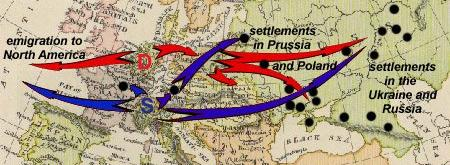
\includegraphics[width=.8\columnwidth]{menno-a}\\\scriptsize
  Courtesy of Paul C. Adams, Department of Geography
  and the Environment, University of Texas at Austin. [1]
\end{center}

\begin{multicols}{2}\small\parskip4pt
\paragraph{Typefaces:}
{\fontfamily{lrm}\selectfont The default typeface in \LaTeX\ is Computer
  Modern, like this.}

{\footnotesize\tabcolsep4pt
\begin{tabular}{@{}l@{\hspace{6pt}}>{\ttfamily}l|l@{\hspace{6pt}}>{\ttfamily}l@{}}
\ff{ptm}Times&mathptmx&\ff{pcr}Courier&courier\\
\ff{ppl}Palatino&mathpazo&\ff{pag}\scriptsize Avant Garde&avant\\
\ff{pbk}Bookman&bookman&\ff{phv}Helvetica&helvet\\
\ff{bch}Charter&charter&\ff{pzc}Zapf Chancery&chancery\\
\ff{put}Utopia&utopia&\ff[OT1]{pnr}Pandora&pandora\\
\ff{pnc}Century&newcent&\ff[U]{yfrak}Fraktur&oldgerm\\
\end{tabular}
}

Dozens of other font packages are available in \TeX\ Live and the \LaTeX\ Font
Catalogue, including mathematics and decorative fonts. Any
Postscript Type~1 font can be configured for \LaTeX.

If you use \XeLaTeX\ and the \textsf{fontspec} package, you can also
use your computer's system fonts as well as those available
with \TeX\ Live.

\colorbox{LightGrey}{\color{black}\begin{minipage}{.965\columnwidth}%
\sffamily\scriptsize\raggedright
Commercial implementations of \TeX\ for Windows with business-level
support are available from Personal \TeX, Inc (PC\TeX); MacKichan
Software, Inc (Scientific Word); Micropress, Inc (V\TeX), and
True\TeX\ Software (True\TeX).\label{comm}
\end{minipage}}

\columnbreak
\textsf{Typefaces continued}

To change font for a word or phrase, use these commands (they can be
nested):

{\small
\begin{tabular}{l@{\enspace}>{\ttfamily\char'134 text}l<{\char'173
      Hello\char'175}@{}>{\ \gives\bgroup}l<{Hello\egroup}}
Italics&it&\itshape\\
Boldface&bf&\bfseries\\
Smallcaps&sc&\ff{cmr}\scshape\\
Sans-serif&sf&\sffamily\\
Monospace&tt&\ttfamily\\
\end{tabular}}

\begingroup\small
\example\verb+\textit{\textbf{\textsf+\linebreak
\verb+{bold italic sans}}}+
\gives{\ff{cmss}\textit{\textbf{bold italic sans}}}
\par\endgroup

Font sizing is automatic for titles, headings, and footnotes. There
are named step-size commands if you need them:

{\scriptsize
\begin{tabular}{>{\ttfamily\char'134}lrrr}
normalsize&10&11&12\\\hline\vrule height1.1em width0pt
tiny&5&6&7\\
scriptsize&6&7&8\\
footnotesize&7&8&9\\
small&9&10&11\\
large&11&12&14\\
Large&12&14&17\rlap*\\
LARGE&14&17\rlap*&20\rlap*\\
huge&17\rlap*&20\rlap*&24\rlap*\\
Huge&20\rlap*&24\rlap*&28\rlap*\\
\end{tabular}
\quad
\rotatebox[origin=c]{90}{\tiny* sizes rounded here to save space}
}

For other sizes, add the special command
{\added\verb+\RequirePackage{fix-cm}+} \emph{before} the 
\verb+\documentclass+ line and use
{\added\verb+\fontsize{+\texttt{\uline{pp}}\verb+}{+\texttt{\uline{bb}}\verb+}\selectfont+}
for the point-size (\textit{pp}) and baseline
(\textit{bb}).

{\sffamily\footnotesize
  Size commands are all \textbf{unscoped} commands, so enclose them \emph{and}
the applicable text in curly braces to stop them affecting the rest
of the document.\par}
For double or 1½ line-spacing (eg in theses) use the \textsf{setspace}
package.

You can use colour palettes in the RGB, CMYK, HTML, and other
colourspaces with the 
\textsf{xcolor} \\package and the\hfil 
\smash{\raisebox{-2ex}{\sffamily\bfseries\Huge\qquad
\textcolor[HTML]{2F50AD}{G}%
\textcolor[HTML]{B32F17}{o}% 
\textcolor[HTML]{F3C20B}{o}%
\textcolor[HTML]{2F50AD}{g}% 
\textcolor[HTML]{48C847}{l}%
\textcolor[HTML]{B32F17}{e}}}%
% web colour for l was 567122
% web colour for o2 was CAB340
\\\verb+\color{+\texttt{\textit{name}}\verb+}+ command.

For verbatim text, use the \verb+\verb+ command or the
\textsf{verbatim} environment, or (better) the \textsf{listings} or
\textsf{fancyvrb} packages, which allow context-sensitive formatting.

\paragraph{Footnotes}\setcounter{footnote}{0} 
You can do footnotes with \verb+\footnote(like this}+.\footnote{Like
  this.} Endnotes too.

\paragraph{Cross-references:}\label{blah} Use the command
\verb+\label{...}+ to add a label to the target, and \verb+\ref{...}+ or
\verb+\pageref{...}+ to refer to it. Make up the labels yourself.

\begingroup\small
\example{...\ttfamily section \verb+\ref{blah}+ on
  p.\\ \verb+\pageref{blah}+.}\gives{...section \ref{blah} on
  p.\thinspace\pageref{blah}}.
\par\endgroup

\paragraph{Citation and reference:} Create your bibliographic database
in BIB\TeX\ format \parencite{bibtex} using \emph{JabRef} or
similar. Each entry \textsc{must} have a unique label
(here `\verb+fi+'):\par\vspace{-\parskip}
\begin{Verbatim}[frame=single,fontsize=\scriptsize,commandchars=!<>]
!added@book{fi,
!added  title = {Formatting Information},
!added  author = {Peter Flynn},
!added  publisher = {Silmaril},
!added  year = {2016}}
\end{Verbatim}
\par\vspace{-\parskip}
Use the
\textsf{biblatex} package to specify the style, and give
the filename of your database:\par\vspace{-\parskip}
\begin{Verbatim}[frame=single,fontsize=\footnotesize,commandchars=!<>]
!added\usepackage[style=apa]{biblatex}
!added\addbibresource{myrefs.bib}
\end{Verbatim}
\par\vspace{-\parskip}
To cite, use \verb+\cite{...}+ (or
\verb+\textcite+ or \verb+\parencite+) with the relevant label:\\ \example{\verb+\textcite{fi}+}\gives{\textcite{fi}}.

\subsubsection{Back matter}
For an index, use the \textsf{makeidx} package and the
\verb+\makeindex+ command with the \verb+\index{...}+
and \verb+\printindex+ commands and the \textsf{makeindex} program.

\nocite{*}
{\defbibheading{shortbib}[References]{\subsection*{#1}}\renewcommand*{\bibfont}{\scriptsize}\setlength{\bibhang}{1em}\urlstyle{tt}\label{refs}\printbibliography[heading=shortbib]}

\colorbox{LightGrey}{\color{black}\begin{minipage}{.965\columnwidth}%
\sffamily\scriptsize\bfseries\raggedright
For information about \LaTeX\ training and consutancy, please contact
Silmaril at \url{latex@silmaril.ie}
\end{minipage}}%
\end{multicols}
\end{document}
      
%</vsg>
% \fi
% \iffalse
%<*docbib>
@book{fi,
  title = {{Formatting Information}},
  subtitle = {{Online {and} {PDF}}},
  author = {Peter Flynn},
  publisher = {Silmaril},
  address = {Cork, Ireland},
  url = {http://latex.silmaril.ie/},
  year = {2018}}

@InProceedings{adams,
  author =       {Paul Adams},
  title =        {{Linguistic Chaos in Montreal}},
  booktitle =    {{Chaos and the City miniconference}},
  year =         2002,
  month =        {11},
  url =          {http://www.utexas.edu/depts/grg/adams/chaos.ppt},
  organization = {University of Texas School of Architecture}}

@Manual{bibtex,
  title =        {{BIB\TeX ing}},
  author =       {Oren Patashnik},
  organization = {\TeX\ Users Group},
  address =      {Portland, RI},
  url = {http://ftp.heanet.ie/pub/CTAN/tex/biblio/bibtex/base/btxdoc.pdf},
  year =         1988}

@Manual{sherington,
  author =       {Sherington, J},
  title =        {{Informative Presentation of Graphs and Statistics}},
  organization = {Statistical Services Centre, University of Reading},
  year =         1998,
  url =          {http://www.reading.ac.uk/ssc/publications/guides/toptgs.htm},
  note =         {4.2, example table}
}

@TechReport{rfc2119,
  author =   {Scott Bradner},
  title =   {{Key words for use in RFCs to Indicate Requirement Levels}},
  institution =  {Internet Engineering Task Force},
  year =   1997,
  number =   {RFC 2119},
  address =   {Fremont, CA},
  url =   {http://www.ietf.org/rfc/rfc2119.txt},
  month =   {3}
}
      
%</docbib>
% \fi
% \Finale

